\hypertarget{_lgm___i_g_r_f_8c}{
\section{/home/mgh/LanlGeoMag/libLanlGeoMag/Lgm\_\-IGRF.c File Reference}
\label{_lgm___i_g_r_f_8c}\index{/home/mgh/LanlGeoMag/libLanlGeoMag/Lgm\_\-IGRF.c@{/home/mgh/LanlGeoMag/libLanlGeoMag/Lgm\_\-IGRF.c}}
}
{\tt \#include \char`\"{}Lgm/Lgm\_\-CTrans.h\char`\"{}}\par
{\tt \#include \char`\"{}Lgm/Lgm\_\-IGRF.h\char`\"{}}\par
{\tt \#include $<$omp.h$>$}\par


Include dependency graph for Lgm\_\-IGRF.c:\nopagebreak
\begin{figure}[H]
\begin{center}
\leavevmode
\includegraphics[width=233pt]{_lgm___i_g_r_f_8c__incl}
\end{center}
\end{figure}
\subsection*{Defines}
\begin{CompactItemize}
\item 
\#define \hyperlink{_lgm___i_g_r_f_8c_cf1c38f71f39386356edb151a131ad11}{TINY}~1.0e-25
\end{CompactItemize}
\subsection*{Functions}
\begin{CompactItemize}
\item 
void \hyperlink{_lgm___i_g_r_f_8c_a25100fb38cb2add3a9f601051299a9a}{Lgm\_\-IGRF} (\hyperlink{struct_lgm___vector}{Lgm\_\-Vector} $\ast$v, \hyperlink{struct_lgm___vector}{Lgm\_\-Vector} $\ast$B, \hyperlink{struct_lgm___c_trans}{Lgm\_\-CTrans} $\ast$c)
\item 
void \hyperlink{_lgm___i_g_r_f_8c_277adeaed44612201277d93893da8812}{\_\-Lgm\_\-IGRF} (\hyperlink{struct_lgm___vector}{Lgm\_\-Vector} $\ast$v, \hyperlink{struct_lgm___vector}{Lgm\_\-Vector} $\ast$B, \hyperlink{struct_lgm___c_trans}{Lgm\_\-CTrans} $\ast$c)
\item 
void \hyperlink{_lgm___i_g_r_f_8c_51daf5cda8c52b2298ae36681a06b841}{\_\-Lgm\_\-IGRF2} (\hyperlink{struct_lgm___vector}{Lgm\_\-Vector} $\ast$v, \hyperlink{struct_lgm___vector}{Lgm\_\-Vector} $\ast$B, \hyperlink{struct_lgm___c_trans}{Lgm\_\-CTrans} $\ast$c)
\item 
void \hyperlink{_lgm___i_g_r_f_8c_008a4169db96afc1d9c25b2913a83940}{\_\-Lgm\_\-IGRF3} (\hyperlink{struct_lgm___vector}{Lgm\_\-Vector} $\ast$v, \hyperlink{struct_lgm___vector}{Lgm\_\-Vector} $\ast$B, \hyperlink{struct_lgm___c_trans}{Lgm\_\-CTrans} $\ast$c)
\item 
void \hyperlink{_lgm___i_g_r_f_8c_1724722babbf7d260eae10d230ded0a3}{\_\-Lgm\_\-IGRF4} (\hyperlink{struct_lgm___vector}{Lgm\_\-Vector} $\ast$v, \hyperlink{struct_lgm___vector}{Lgm\_\-Vector} $\ast$B, \hyperlink{struct_lgm___c_trans}{Lgm\_\-CTrans} $\ast$c)
\item 
void \hyperlink{_lgm___i_g_r_f_8c_401083eedac0b8fc82e4ab20927d499a}{Lgm\_\-InitPnm} (double ct, double st, double R\mbox{[}13\mbox{]}\mbox{[}13\mbox{]}, double P\mbox{[}13\mbox{]}\mbox{[}13\mbox{]}, double dP\mbox{[}13\mbox{]}\mbox{[}13\mbox{]}, int N, \hyperlink{struct_lgm___c_trans}{Lgm\_\-CTrans} $\ast$c)
\item 
void \hyperlink{_lgm___i_g_r_f_8c_22d8045554f6d6dd27b725f9c73e68ef}{Lgm\_\-InitdPnm} (double P\mbox{[}13\mbox{]}\mbox{[}13\mbox{]}, double dP\mbox{[}13\mbox{]}\mbox{[}13\mbox{]}, int N, \hyperlink{struct_lgm___c_trans}{Lgm\_\-CTrans} $\ast$c)
\item 
void \hyperlink{_lgm___i_g_r_f_8c_525177976ecea85ebc006e0a61b3fbb3}{Lgm\_\-InitSqrtFuncs} (double SqrtNM1\mbox{[}13\mbox{]}\mbox{[}13\mbox{]}, double SqrtNM2\mbox{[}13\mbox{]}\mbox{[}13\mbox{]}, int N)
\item 
double \hyperlink{_lgm___i_g_r_f_8c_a650901117046cbe022b3dc771f098d5}{Lgm\_\-Factorial} (int k)
\item 
void \hyperlink{_lgm___i_g_r_f_8c_83af74ea368f0c443c59eb76388daa2c}{Lgm\_\-InitTrigmp} (double cp, double sp, double $\ast$Cmp, double $\ast$Smp, int N)
\item 
void \hyperlink{_lgm___i_g_r_f_8c_1754fc8886cfcd3bf3e97dfc38767190}{Lgm\_\-InitS} (double S\mbox{[}13\mbox{]}\mbox{[}13\mbox{]}, int N)
\item 
void \hyperlink{_lgm___i_g_r_f_8c_09e15d914fd48a3df511a033e6eed606}{Lgm\_\-InitK} (double K\mbox{[}13\mbox{]}\mbox{[}13\mbox{]}, int N)
\item 
void \hyperlink{_lgm___i_g_r_f_8c_6cda667f1a74bdd3549eeb54f805755e}{Lgm\_\-InitIGRF} (double g\mbox{[}13\mbox{]}\mbox{[}13\mbox{]}, double h\mbox{[}13\mbox{]}\mbox{[}13\mbox{]}, int N, int Flag, \hyperlink{struct_lgm___c_trans}{Lgm\_\-CTrans} $\ast$c)
\item 
void \hyperlink{_lgm___i_g_r_f_8c_5f539fb0ce5cd439a515a3ab044ea541}{Lgm\_\-PolFunInt} (double $\ast$xa, double $\ast$ya, int n, double x, double $\ast$y, double $\ast$dy)
\item 
void \hyperlink{_lgm___i_g_r_f_8c_6a1227953eb4946e200ce05ce8d897f3}{Lgm\_\-RatFunInt} (double $\ast$xa, double $\ast$ya, int n, double x, double $\ast$y, double $\ast$dy)
\end{CompactItemize}


\subsection{Define Documentation}
\hypertarget{_lgm___i_g_r_f_8c_cf1c38f71f39386356edb151a131ad11}{
\index{Lgm\_\-IGRF.c@{Lgm\_\-IGRF.c}!TINY@{TINY}}
\index{TINY@{TINY}!Lgm_IGRF.c@{Lgm\_\-IGRF.c}}
\subsubsection[{TINY}]{\setlength{\rightskip}{0pt plus 5cm}\#define TINY~1.0e-25}}
\label{_lgm___i_g_r_f_8c_cf1c38f71f39386356edb151a131ad11}




Definition at line 39 of file Lgm\_\-IGRF.c.

\subsection{Function Documentation}
\hypertarget{_lgm___i_g_r_f_8c_a25100fb38cb2add3a9f601051299a9a}{
\index{Lgm\_\-IGRF.c@{Lgm\_\-IGRF.c}!Lgm\_\-IGRF@{Lgm\_\-IGRF}}
\index{Lgm\_\-IGRF@{Lgm\_\-IGRF}!Lgm_IGRF.c@{Lgm\_\-IGRF.c}}
\subsubsection[{Lgm\_\-IGRF}]{\setlength{\rightskip}{0pt plus 5cm}void Lgm\_\-IGRF ({\bf Lgm\_\-Vector} $\ast$ {\em v}, \/  {\bf Lgm\_\-Vector} $\ast$ {\em B}, \/  {\bf Lgm\_\-CTrans} $\ast$ {\em c})}}
\label{_lgm___i_g_r_f_8c_a25100fb38cb2add3a9f601051299a9a}




Definition at line 46 of file Lgm\_\-IGRF.c.

Here is the call graph for this function:\nopagebreak
\begin{figure}[H]
\begin{center}
\leavevmode
\includegraphics[width=173pt]{_lgm___i_g_r_f_8c_a25100fb38cb2add3a9f601051299a9a_cgraph}
\end{center}
\end{figure}


Here is the caller graph for this function:\nopagebreak
\begin{figure}[H]
\begin{center}
\leavevmode
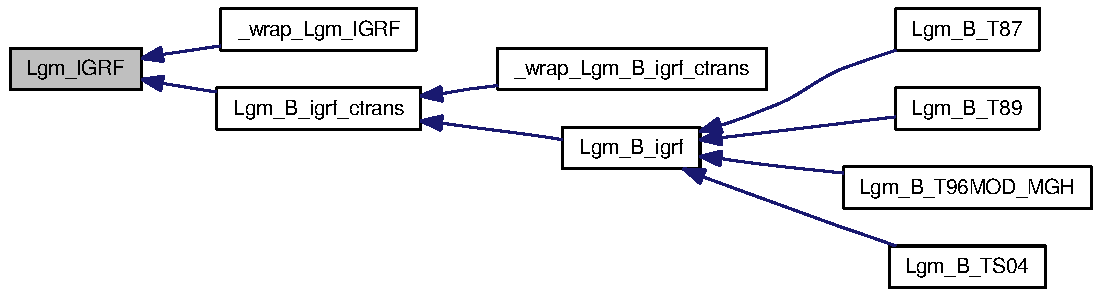
\includegraphics[width=282pt]{_lgm___i_g_r_f_8c_a25100fb38cb2add3a9f601051299a9a_icgraph}
\end{center}
\end{figure}
\hypertarget{_lgm___i_g_r_f_8c_277adeaed44612201277d93893da8812}{
\index{Lgm\_\-IGRF.c@{Lgm\_\-IGRF.c}!\_\-Lgm\_\-IGRF@{\_\-Lgm\_\-IGRF}}
\index{\_\-Lgm\_\-IGRF@{\_\-Lgm\_\-IGRF}!Lgm_IGRF.c@{Lgm\_\-IGRF.c}}
\subsubsection[{\_\-Lgm\_\-IGRF}]{\setlength{\rightskip}{0pt plus 5cm}void \_\-Lgm\_\-IGRF ({\bf Lgm\_\-Vector} $\ast$ {\em v}, \/  {\bf Lgm\_\-Vector} $\ast$ {\em B}, \/  {\bf Lgm\_\-CTrans} $\ast$ {\em c})}}
\label{_lgm___i_g_r_f_8c_277adeaed44612201277d93893da8812}




Definition at line 84 of file Lgm\_\-IGRF.c.

Here is the call graph for this function:\nopagebreak
\begin{figure}[H]
\begin{center}
\leavevmode
\includegraphics[width=243pt]{_lgm___i_g_r_f_8c_277adeaed44612201277d93893da8812_cgraph}
\end{center}
\end{figure}


Here is the caller graph for this function:\nopagebreak
\begin{figure}[H]
\begin{center}
\leavevmode
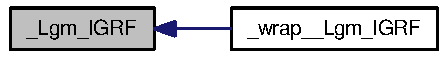
\includegraphics[width=125pt]{_lgm___i_g_r_f_8c_277adeaed44612201277d93893da8812_icgraph}
\end{center}
\end{figure}
\hypertarget{_lgm___i_g_r_f_8c_51daf5cda8c52b2298ae36681a06b841}{
\index{Lgm\_\-IGRF.c@{Lgm\_\-IGRF.c}!\_\-Lgm\_\-IGRF2@{\_\-Lgm\_\-IGRF2}}
\index{\_\-Lgm\_\-IGRF2@{\_\-Lgm\_\-IGRF2}!Lgm_IGRF.c@{Lgm\_\-IGRF.c}}
\subsubsection[{\_\-Lgm\_\-IGRF2}]{\setlength{\rightskip}{0pt plus 5cm}void \_\-Lgm\_\-IGRF2 ({\bf Lgm\_\-Vector} $\ast$ {\em v}, \/  {\bf Lgm\_\-Vector} $\ast$ {\em B}, \/  {\bf Lgm\_\-CTrans} $\ast$ {\em c})}}
\label{_lgm___i_g_r_f_8c_51daf5cda8c52b2298ae36681a06b841}




Definition at line 211 of file Lgm\_\-IGRF.c.

Here is the call graph for this function:\nopagebreak
\begin{figure}[H]
\begin{center}
\leavevmode
\includegraphics[width=119pt]{_lgm___i_g_r_f_8c_51daf5cda8c52b2298ae36681a06b841_cgraph}
\end{center}
\end{figure}
\hypertarget{_lgm___i_g_r_f_8c_008a4169db96afc1d9c25b2913a83940}{
\index{Lgm\_\-IGRF.c@{Lgm\_\-IGRF.c}!\_\-Lgm\_\-IGRF3@{\_\-Lgm\_\-IGRF3}}
\index{\_\-Lgm\_\-IGRF3@{\_\-Lgm\_\-IGRF3}!Lgm_IGRF.c@{Lgm\_\-IGRF.c}}
\subsubsection[{\_\-Lgm\_\-IGRF3}]{\setlength{\rightskip}{0pt plus 5cm}void \_\-Lgm\_\-IGRF3 ({\bf Lgm\_\-Vector} $\ast$ {\em v}, \/  {\bf Lgm\_\-Vector} $\ast$ {\em B}, \/  {\bf Lgm\_\-CTrans} $\ast$ {\em c})}}
\label{_lgm___i_g_r_f_8c_008a4169db96afc1d9c25b2913a83940}




Definition at line 354 of file Lgm\_\-IGRF.c.

Here is the call graph for this function:\nopagebreak
\begin{figure}[H]
\begin{center}
\leavevmode
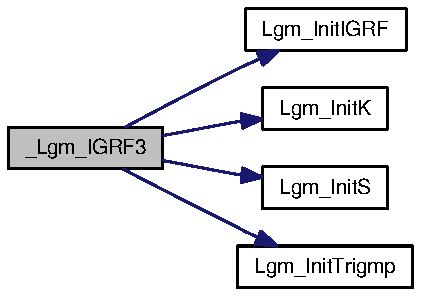
\includegraphics[width=119pt]{_lgm___i_g_r_f_8c_008a4169db96afc1d9c25b2913a83940_cgraph}
\end{center}
\end{figure}
\hypertarget{_lgm___i_g_r_f_8c_1724722babbf7d260eae10d230ded0a3}{
\index{Lgm\_\-IGRF.c@{Lgm\_\-IGRF.c}!\_\-Lgm\_\-IGRF4@{\_\-Lgm\_\-IGRF4}}
\index{\_\-Lgm\_\-IGRF4@{\_\-Lgm\_\-IGRF4}!Lgm_IGRF.c@{Lgm\_\-IGRF.c}}
\subsubsection[{\_\-Lgm\_\-IGRF4}]{\setlength{\rightskip}{0pt plus 5cm}void \_\-Lgm\_\-IGRF4 ({\bf Lgm\_\-Vector} $\ast$ {\em v}, \/  {\bf Lgm\_\-Vector} $\ast$ {\em B}, \/  {\bf Lgm\_\-CTrans} $\ast$ {\em c})}}
\label{_lgm___i_g_r_f_8c_1724722babbf7d260eae10d230ded0a3}




Definition at line 527 of file Lgm\_\-IGRF.c.

Here is the call graph for this function:\nopagebreak
\begin{figure}[H]
\begin{center}
\leavevmode
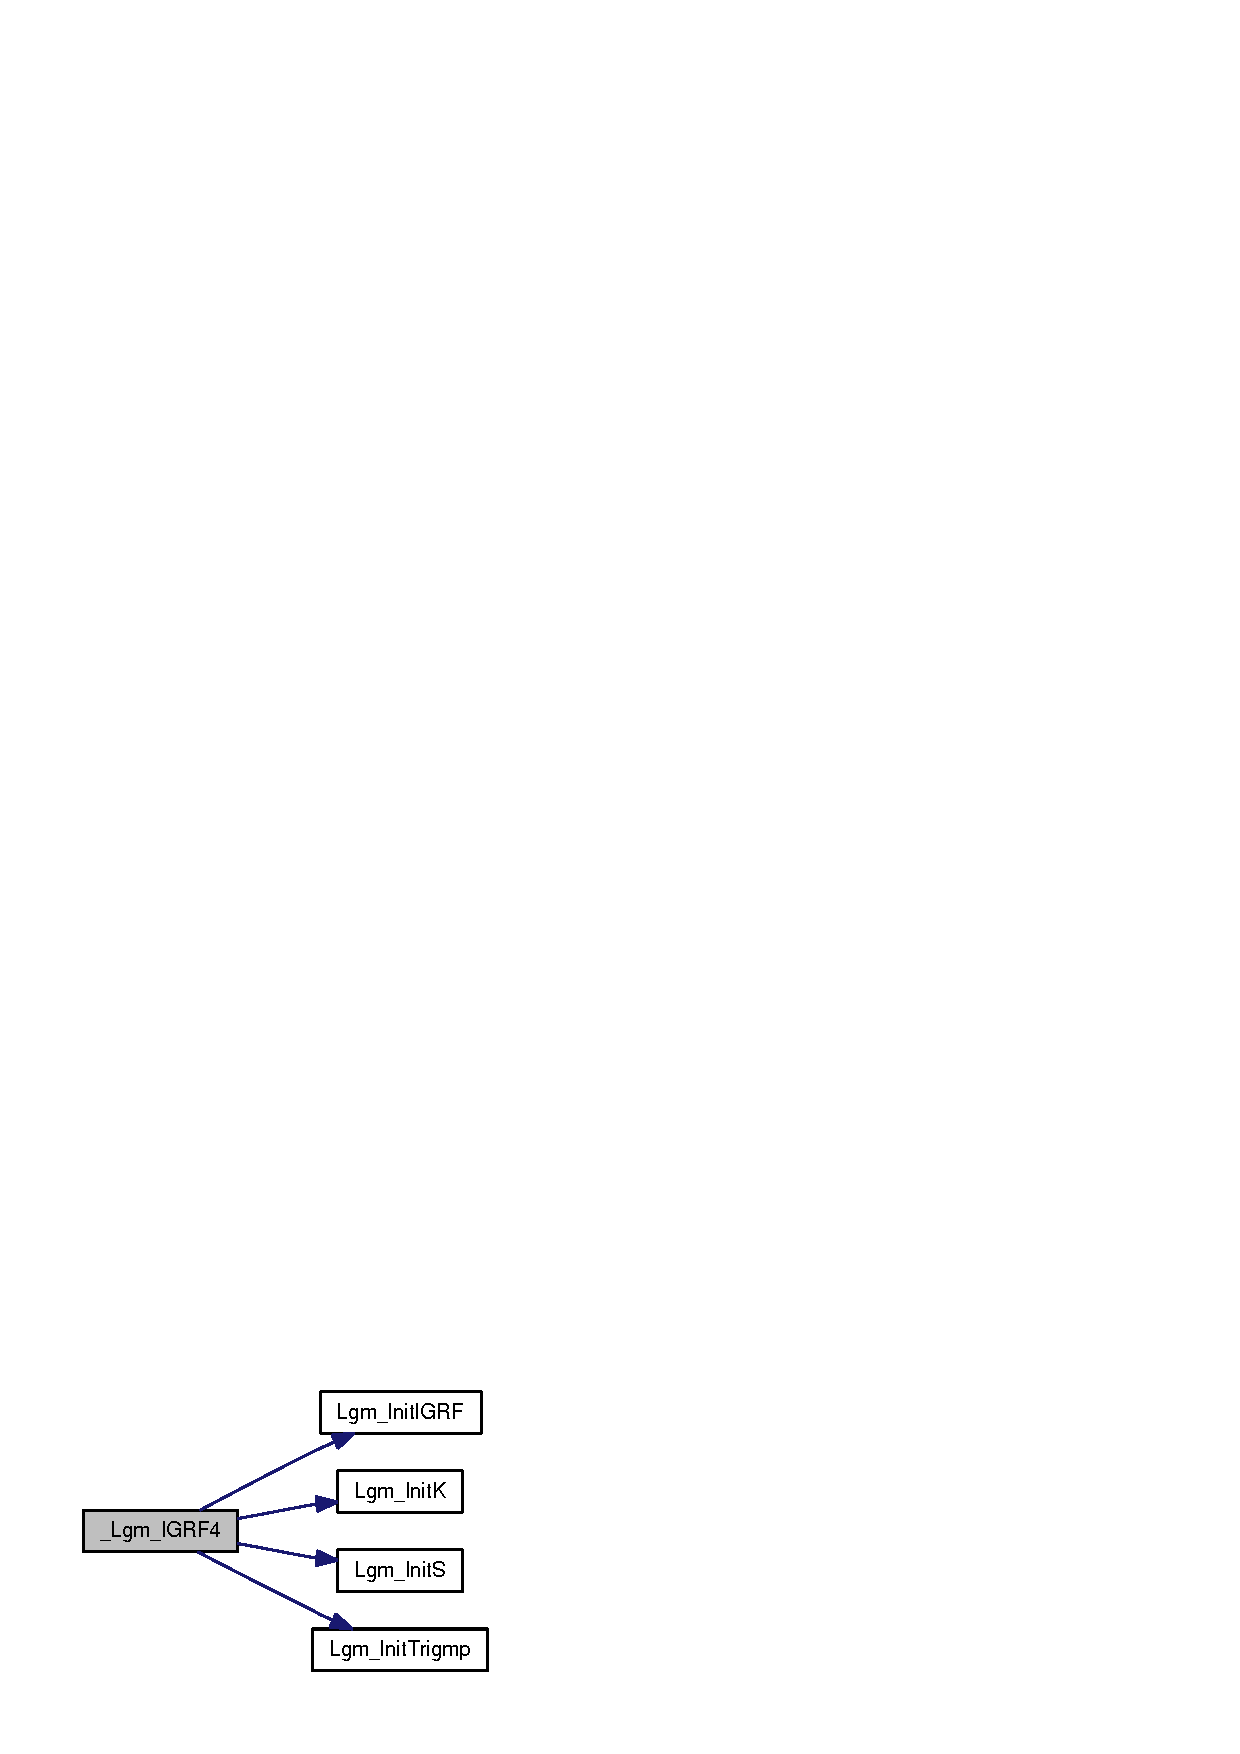
\includegraphics[width=119pt]{_lgm___i_g_r_f_8c_1724722babbf7d260eae10d230ded0a3_cgraph}
\end{center}
\end{figure}


Here is the caller graph for this function:\nopagebreak
\begin{figure}[H]
\begin{center}
\leavevmode
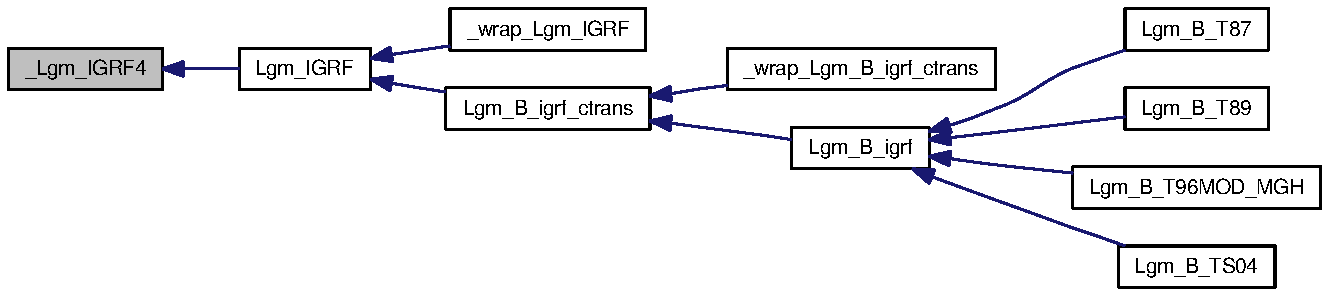
\includegraphics[width=337pt]{_lgm___i_g_r_f_8c_1724722babbf7d260eae10d230ded0a3_icgraph}
\end{center}
\end{figure}
\hypertarget{_lgm___i_g_r_f_8c_401083eedac0b8fc82e4ab20927d499a}{
\index{Lgm\_\-IGRF.c@{Lgm\_\-IGRF.c}!Lgm\_\-InitPnm@{Lgm\_\-InitPnm}}
\index{Lgm\_\-InitPnm@{Lgm\_\-InitPnm}!Lgm_IGRF.c@{Lgm\_\-IGRF.c}}
\subsubsection[{Lgm\_\-InitPnm}]{\setlength{\rightskip}{0pt plus 5cm}void Lgm\_\-InitPnm (double {\em ct}, \/  double {\em st}, \/  double {\em R}\mbox{[}13\mbox{]}\mbox{[}13\mbox{]}, \/  double {\em P}\mbox{[}13\mbox{]}\mbox{[}13\mbox{]}, \/  double {\em dP}\mbox{[}13\mbox{]}\mbox{[}13\mbox{]}, \/  int {\em N}, \/  {\bf Lgm\_\-CTrans} $\ast$ {\em c})}}
\label{_lgm___i_g_r_f_8c_401083eedac0b8fc82e4ab20927d499a}




Definition at line 677 of file Lgm\_\-IGRF.c.

Here is the call graph for this function:\nopagebreak
\begin{figure}[H]
\begin{center}
\leavevmode
\includegraphics[width=185pt]{_lgm___i_g_r_f_8c_401083eedac0b8fc82e4ab20927d499a_cgraph}
\end{center}
\end{figure}


Here is the caller graph for this function:\nopagebreak
\begin{figure}[H]
\begin{center}
\leavevmode
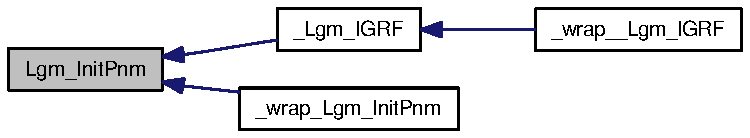
\includegraphics[width=198pt]{_lgm___i_g_r_f_8c_401083eedac0b8fc82e4ab20927d499a_icgraph}
\end{center}
\end{figure}
\hypertarget{_lgm___i_g_r_f_8c_22d8045554f6d6dd27b725f9c73e68ef}{
\index{Lgm\_\-IGRF.c@{Lgm\_\-IGRF.c}!Lgm\_\-InitdPnm@{Lgm\_\-InitdPnm}}
\index{Lgm\_\-InitdPnm@{Lgm\_\-InitdPnm}!Lgm_IGRF.c@{Lgm\_\-IGRF.c}}
\subsubsection[{Lgm\_\-InitdPnm}]{\setlength{\rightskip}{0pt plus 5cm}void Lgm\_\-InitdPnm (double {\em P}\mbox{[}13\mbox{]}\mbox{[}13\mbox{]}, \/  double {\em dP}\mbox{[}13\mbox{]}\mbox{[}13\mbox{]}, \/  int {\em N}, \/  {\bf Lgm\_\-CTrans} $\ast$ {\em c})}}
\label{_lgm___i_g_r_f_8c_22d8045554f6d6dd27b725f9c73e68ef}




Definition at line 808 of file Lgm\_\-IGRF.c.

Here is the call graph for this function:\nopagebreak
\begin{figure}[H]
\begin{center}
\leavevmode
\includegraphics[width=130pt]{_lgm___i_g_r_f_8c_22d8045554f6d6dd27b725f9c73e68ef_cgraph}
\end{center}
\end{figure}


Here is the caller graph for this function:\nopagebreak
\begin{figure}[H]
\begin{center}
\leavevmode
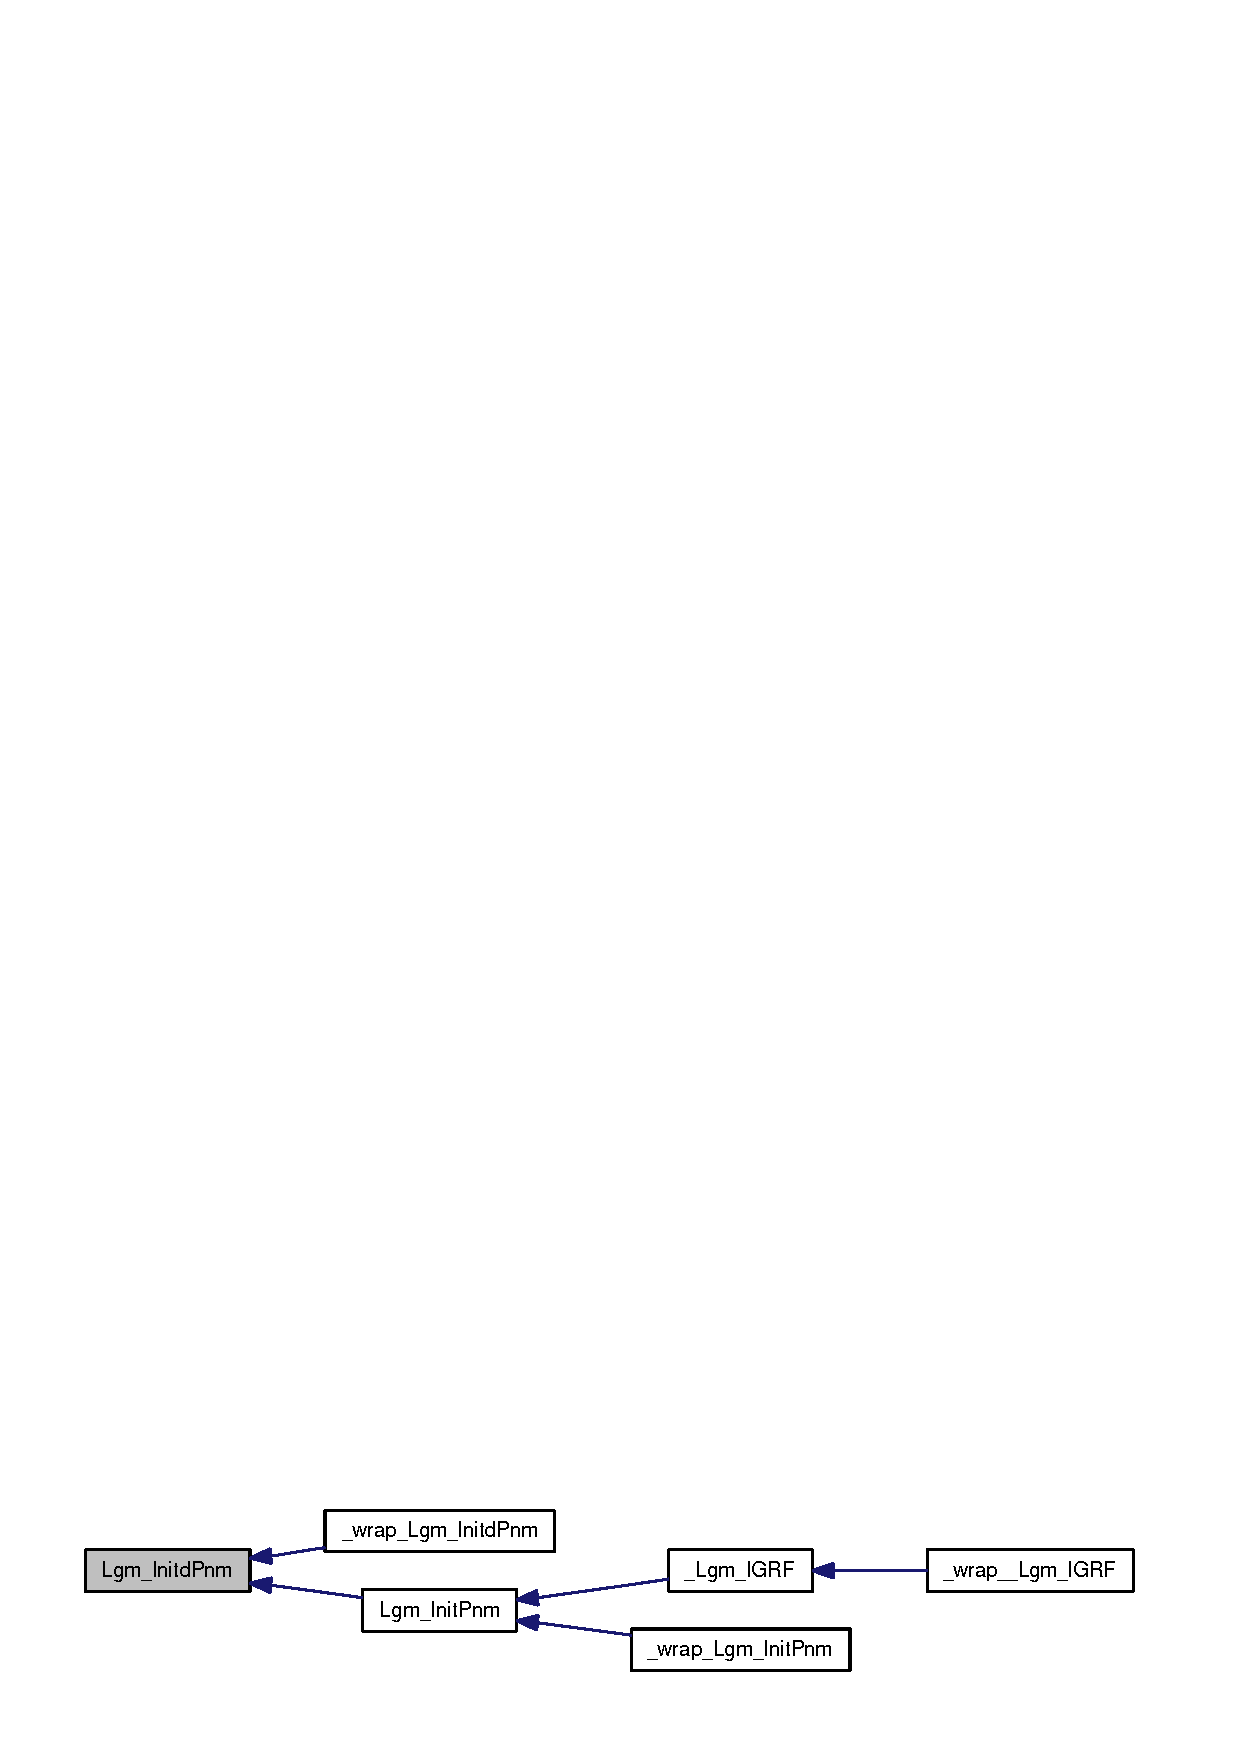
\includegraphics[width=274pt]{_lgm___i_g_r_f_8c_22d8045554f6d6dd27b725f9c73e68ef_icgraph}
\end{center}
\end{figure}
\hypertarget{_lgm___i_g_r_f_8c_525177976ecea85ebc006e0a61b3fbb3}{
\index{Lgm\_\-IGRF.c@{Lgm\_\-IGRF.c}!Lgm\_\-InitSqrtFuncs@{Lgm\_\-InitSqrtFuncs}}
\index{Lgm\_\-InitSqrtFuncs@{Lgm\_\-InitSqrtFuncs}!Lgm_IGRF.c@{Lgm\_\-IGRF.c}}
\subsubsection[{Lgm\_\-InitSqrtFuncs}]{\setlength{\rightskip}{0pt plus 5cm}void Lgm\_\-InitSqrtFuncs (double {\em SqrtNM1}\mbox{[}13\mbox{]}\mbox{[}13\mbox{]}, \/  double {\em SqrtNM2}\mbox{[}13\mbox{]}\mbox{[}13\mbox{]}, \/  int {\em N})}}
\label{_lgm___i_g_r_f_8c_525177976ecea85ebc006e0a61b3fbb3}




Definition at line 848 of file Lgm\_\-IGRF.c.

Here is the caller graph for this function:\nopagebreak
\begin{figure}[H]
\begin{center}
\leavevmode
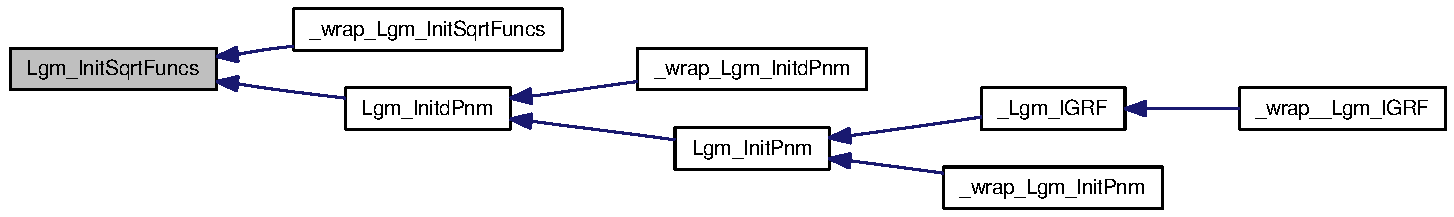
\includegraphics[width=367pt]{_lgm___i_g_r_f_8c_525177976ecea85ebc006e0a61b3fbb3_icgraph}
\end{center}
\end{figure}
\hypertarget{_lgm___i_g_r_f_8c_a650901117046cbe022b3dc771f098d5}{
\index{Lgm\_\-IGRF.c@{Lgm\_\-IGRF.c}!Lgm\_\-Factorial@{Lgm\_\-Factorial}}
\index{Lgm\_\-Factorial@{Lgm\_\-Factorial}!Lgm_IGRF.c@{Lgm\_\-IGRF.c}}
\subsubsection[{Lgm\_\-Factorial}]{\setlength{\rightskip}{0pt plus 5cm}double Lgm\_\-Factorial (int {\em k})}}
\label{_lgm___i_g_r_f_8c_a650901117046cbe022b3dc771f098d5}




Definition at line 879 of file Lgm\_\-IGRF.c.

Here is the caller graph for this function:\nopagebreak
\begin{figure}[H]
\begin{center}
\leavevmode
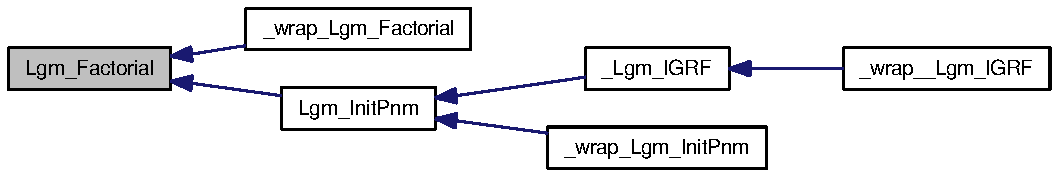
\includegraphics[width=272pt]{_lgm___i_g_r_f_8c_a650901117046cbe022b3dc771f098d5_icgraph}
\end{center}
\end{figure}
\hypertarget{_lgm___i_g_r_f_8c_83af74ea368f0c443c59eb76388daa2c}{
\index{Lgm\_\-IGRF.c@{Lgm\_\-IGRF.c}!Lgm\_\-InitTrigmp@{Lgm\_\-InitTrigmp}}
\index{Lgm\_\-InitTrigmp@{Lgm\_\-InitTrigmp}!Lgm_IGRF.c@{Lgm\_\-IGRF.c}}
\subsubsection[{Lgm\_\-InitTrigmp}]{\setlength{\rightskip}{0pt plus 5cm}void Lgm\_\-InitTrigmp (double {\em cp}, \/  double {\em sp}, \/  double $\ast$ {\em Cmp}, \/  double $\ast$ {\em Smp}, \/  int {\em N})}}
\label{_lgm___i_g_r_f_8c_83af74ea368f0c443c59eb76388daa2c}




Definition at line 900 of file Lgm\_\-IGRF.c.

Here is the caller graph for this function:\nopagebreak
\begin{figure}[H]
\begin{center}
\leavevmode
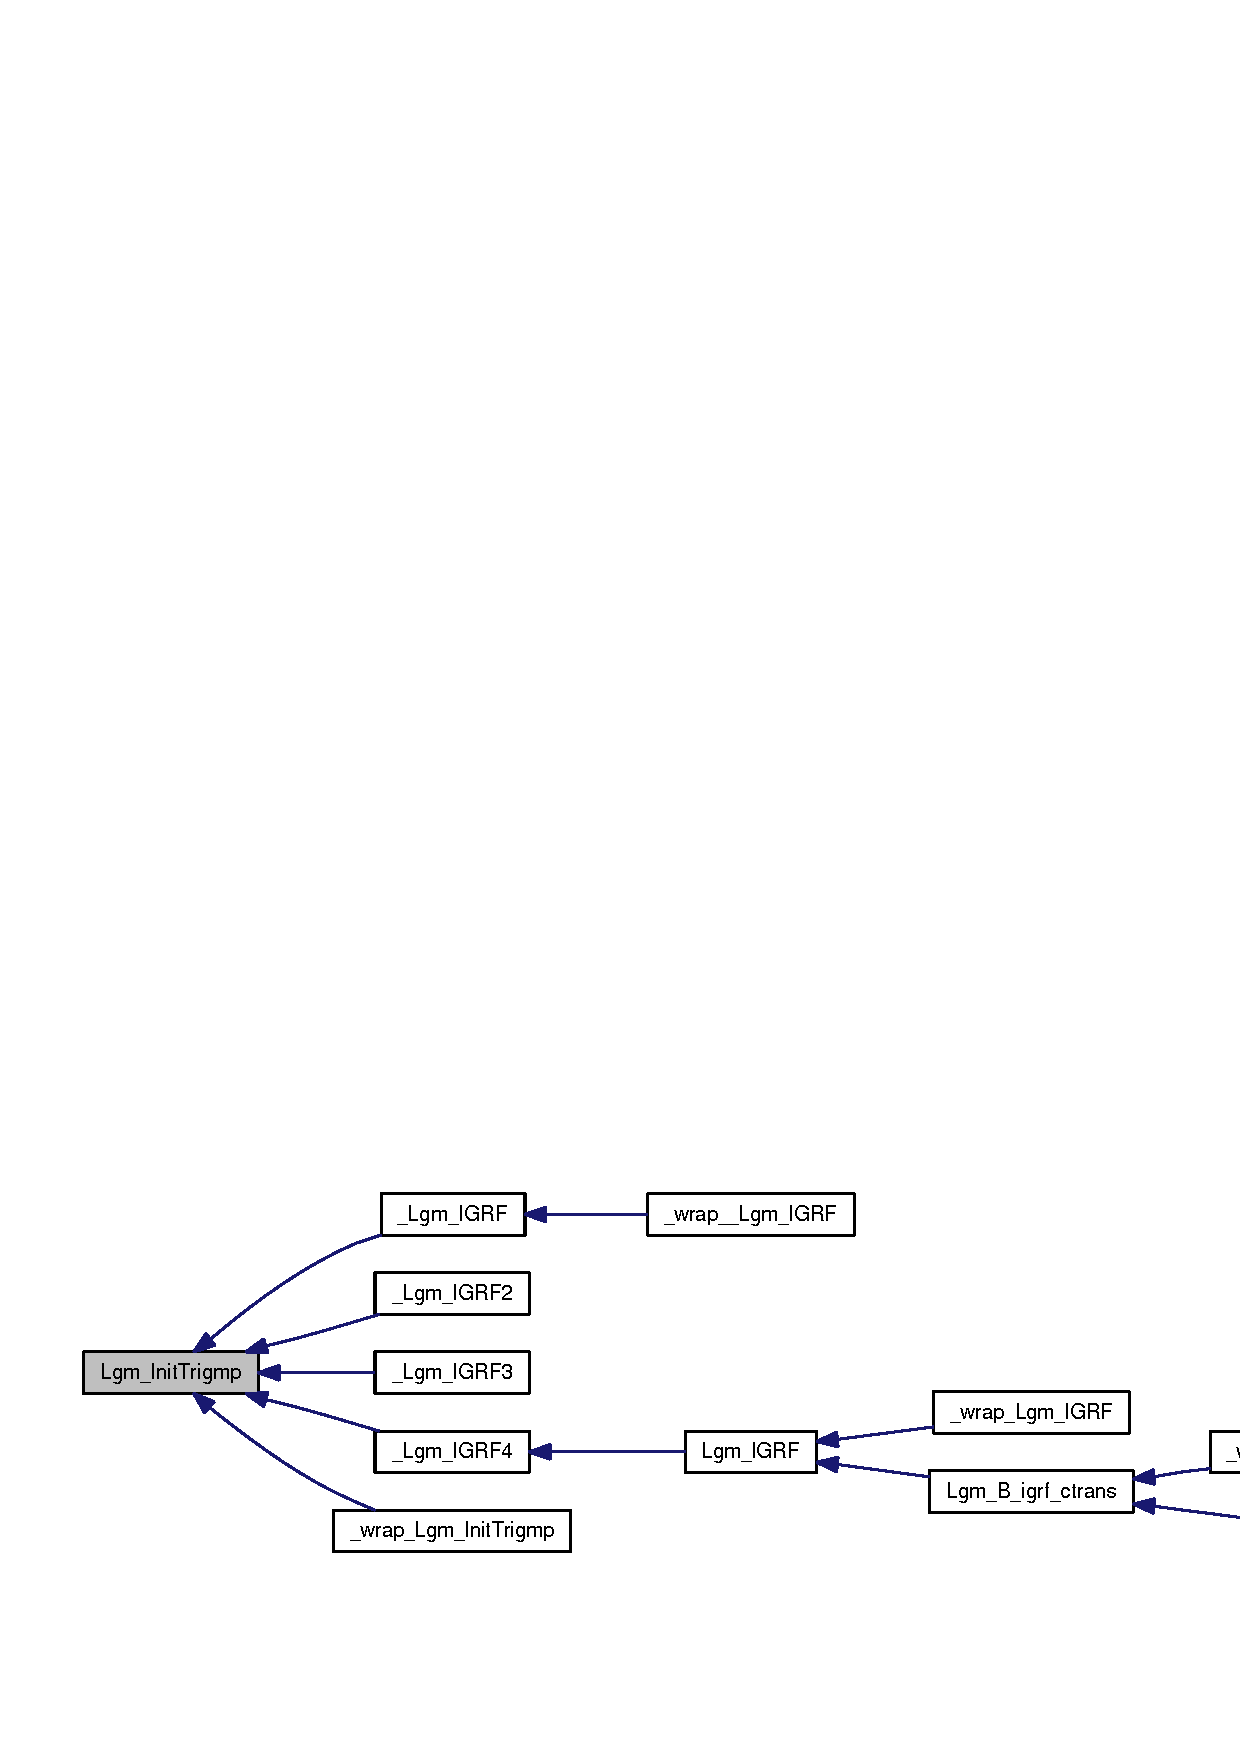
\includegraphics[width=420pt]{_lgm___i_g_r_f_8c_83af74ea368f0c443c59eb76388daa2c_icgraph}
\end{center}
\end{figure}
\hypertarget{_lgm___i_g_r_f_8c_1754fc8886cfcd3bf3e97dfc38767190}{
\index{Lgm\_\-IGRF.c@{Lgm\_\-IGRF.c}!Lgm\_\-InitS@{Lgm\_\-InitS}}
\index{Lgm\_\-InitS@{Lgm\_\-InitS}!Lgm_IGRF.c@{Lgm\_\-IGRF.c}}
\subsubsection[{Lgm\_\-InitS}]{\setlength{\rightskip}{0pt plus 5cm}void Lgm\_\-InitS (double {\em S}\mbox{[}13\mbox{]}\mbox{[}13\mbox{]}, \/  int {\em N})}}
\label{_lgm___i_g_r_f_8c_1754fc8886cfcd3bf3e97dfc38767190}




Definition at line 925 of file Lgm\_\-IGRF.c.

Here is the caller graph for this function:\nopagebreak
\begin{figure}[H]
\begin{center}
\leavevmode
\includegraphics[width=385pt]{_lgm___i_g_r_f_8c_1754fc8886cfcd3bf3e97dfc38767190_icgraph}
\end{center}
\end{figure}
\hypertarget{_lgm___i_g_r_f_8c_09e15d914fd48a3df511a033e6eed606}{
\index{Lgm\_\-IGRF.c@{Lgm\_\-IGRF.c}!Lgm\_\-InitK@{Lgm\_\-InitK}}
\index{Lgm\_\-InitK@{Lgm\_\-InitK}!Lgm_IGRF.c@{Lgm\_\-IGRF.c}}
\subsubsection[{Lgm\_\-InitK}]{\setlength{\rightskip}{0pt plus 5cm}void Lgm\_\-InitK (double {\em K}\mbox{[}13\mbox{]}\mbox{[}13\mbox{]}, \/  int {\em N})}}
\label{_lgm___i_g_r_f_8c_09e15d914fd48a3df511a033e6eed606}




Definition at line 960 of file Lgm\_\-IGRF.c.

Here is the caller graph for this function:\nopagebreak
\begin{figure}[H]
\begin{center}
\leavevmode
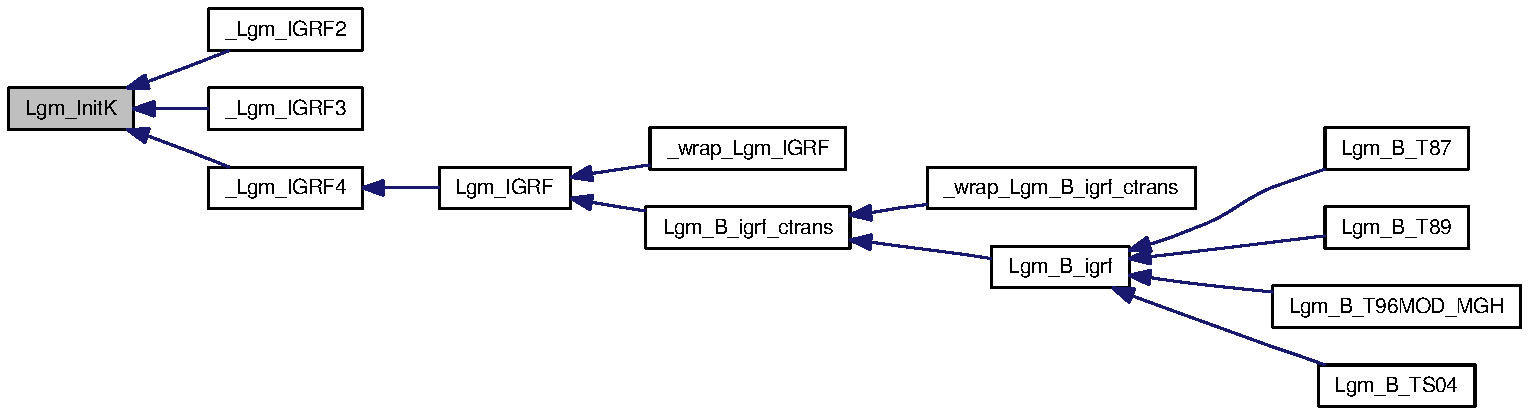
\includegraphics[width=385pt]{_lgm___i_g_r_f_8c_09e15d914fd48a3df511a033e6eed606_icgraph}
\end{center}
\end{figure}
\hypertarget{_lgm___i_g_r_f_8c_6cda667f1a74bdd3549eeb54f805755e}{
\index{Lgm\_\-IGRF.c@{Lgm\_\-IGRF.c}!Lgm\_\-InitIGRF@{Lgm\_\-InitIGRF}}
\index{Lgm\_\-InitIGRF@{Lgm\_\-InitIGRF}!Lgm_IGRF.c@{Lgm\_\-IGRF.c}}
\subsubsection[{Lgm\_\-InitIGRF}]{\setlength{\rightskip}{0pt plus 5cm}void Lgm\_\-InitIGRF (double {\em g}\mbox{[}13\mbox{]}\mbox{[}13\mbox{]}, \/  double {\em h}\mbox{[}13\mbox{]}\mbox{[}13\mbox{]}, \/  int {\em N}, \/  int {\em Flag}, \/  {\bf Lgm\_\-CTrans} $\ast$ {\em c})}}
\label{_lgm___i_g_r_f_8c_6cda667f1a74bdd3549eeb54f805755e}




Definition at line 982 of file Lgm\_\-IGRF.c.

Here is the caller graph for this function:\nopagebreak
\begin{figure}[H]
\begin{center}
\leavevmode
\includegraphics[width=420pt]{_lgm___i_g_r_f_8c_6cda667f1a74bdd3549eeb54f805755e_icgraph}
\end{center}
\end{figure}
\hypertarget{_lgm___i_g_r_f_8c_5f539fb0ce5cd439a515a3ab044ea541}{
\index{Lgm\_\-IGRF.c@{Lgm\_\-IGRF.c}!Lgm\_\-PolFunInt@{Lgm\_\-PolFunInt}}
\index{Lgm\_\-PolFunInt@{Lgm\_\-PolFunInt}!Lgm_IGRF.c@{Lgm\_\-IGRF.c}}
\subsubsection[{Lgm\_\-PolFunInt}]{\setlength{\rightskip}{0pt plus 5cm}void Lgm\_\-PolFunInt (double $\ast$ {\em xa}, \/  double $\ast$ {\em ya}, \/  int {\em n}, \/  double {\em x}, \/  double $\ast$ {\em y}, \/  double $\ast$ {\em dy})}}
\label{_lgm___i_g_r_f_8c_5f539fb0ce5cd439a515a3ab044ea541}




Definition at line 1086 of file Lgm\_\-IGRF.c.

Here is the caller graph for this function:\nopagebreak
\begin{figure}[H]
\begin{center}
\leavevmode
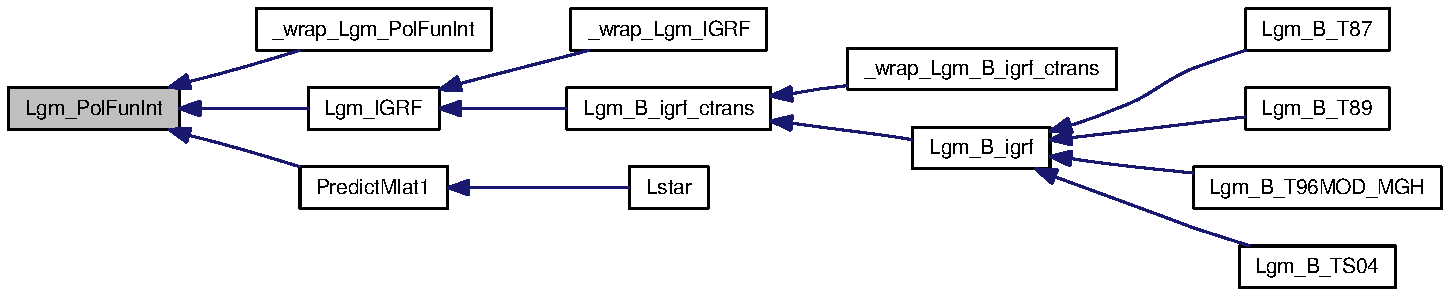
\includegraphics[width=366pt]{_lgm___i_g_r_f_8c_5f539fb0ce5cd439a515a3ab044ea541_icgraph}
\end{center}
\end{figure}
\hypertarget{_lgm___i_g_r_f_8c_6a1227953eb4946e200ce05ce8d897f3}{
\index{Lgm\_\-IGRF.c@{Lgm\_\-IGRF.c}!Lgm\_\-RatFunInt@{Lgm\_\-RatFunInt}}
\index{Lgm\_\-RatFunInt@{Lgm\_\-RatFunInt}!Lgm_IGRF.c@{Lgm\_\-IGRF.c}}
\subsubsection[{Lgm\_\-RatFunInt}]{\setlength{\rightskip}{0pt plus 5cm}void Lgm\_\-RatFunInt (double $\ast$ {\em xa}, \/  double $\ast$ {\em ya}, \/  int {\em n}, \/  double {\em x}, \/  double $\ast$ {\em y}, \/  double $\ast$ {\em dy})}}
\label{_lgm___i_g_r_f_8c_6a1227953eb4946e200ce05ce8d897f3}




Definition at line 1126 of file Lgm\_\-IGRF.c.

Here is the caller graph for this function:\nopagebreak
\begin{figure}[H]
\begin{center}
\leavevmode
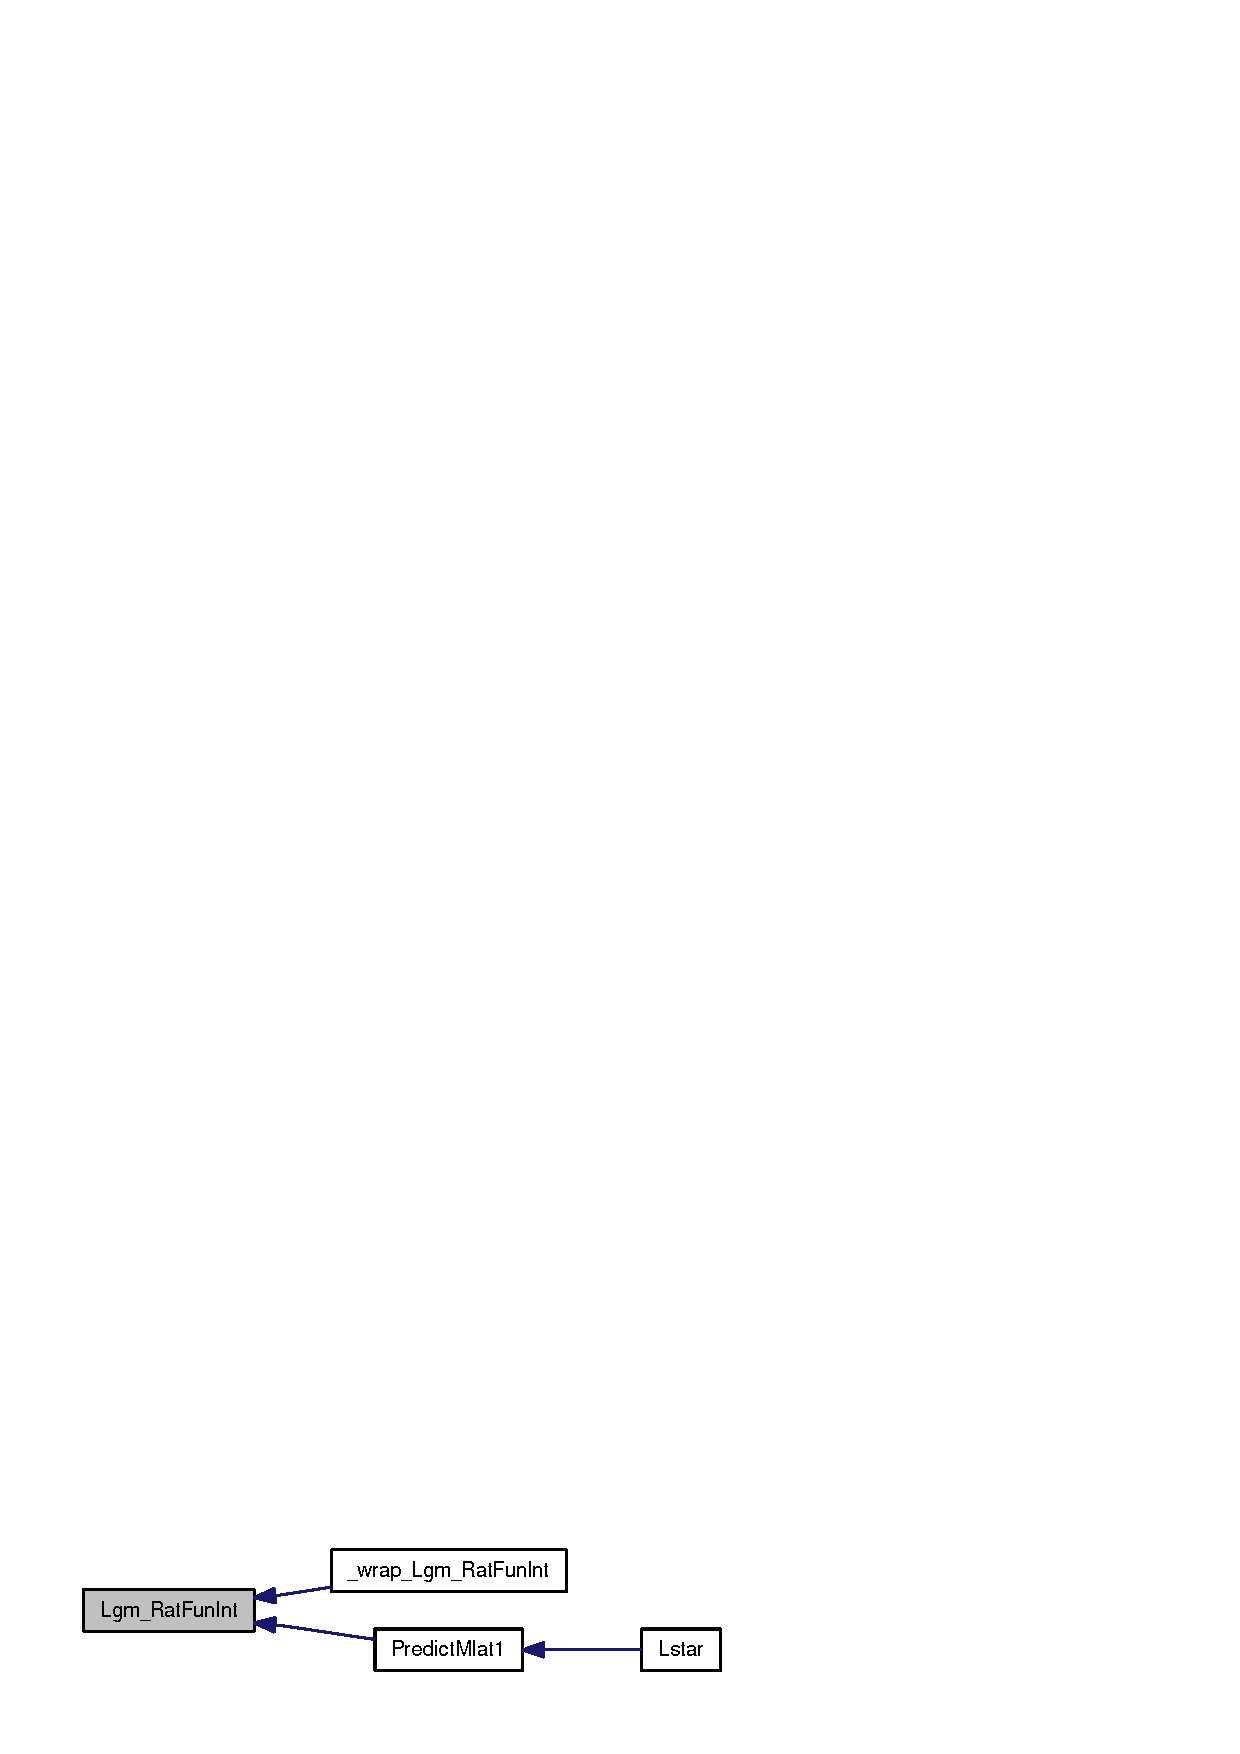
\includegraphics[width=175pt]{_lgm___i_g_r_f_8c_6a1227953eb4946e200ce05ce8d897f3_icgraph}
\end{center}
\end{figure}
